\documentclass[12pt,a4paper]{article}

% --- Paquetes de idioma y codificación ---
\usepackage[utf8]{inputenc}
\usepackage[T1]{fontenc}
\usepackage[spanish,es-tabla]{babel}

% --- Margenes y diseño de página ---
\usepackage[margin=2.5cm]{geometry}
\usepackage{setspace}
\onehalfspacing

% --- Tipografía y color ---
\usepackage{lmodern}
\usepackage{xcolor}
\definecolor{codegreen}{rgb}{0,0.6,0}
\definecolor{codegray}{rgb}{0.5,0.5,0.5}
\definecolor{codepurple}{rgb}{0.58,0,0.82}
\definecolor{backcolour}{rgb}{0.96,0.96,0.96}
\definecolor{primaryblue}{RGB}{0, 78, 152}

% --- Paquetes para código y tablas ---
\usepackage{listings}
\usepackage{booktabs}
\usepackage{tabularx}
\usepackage{longtable}
\usepackage{array}

% --- Paquetes para gráficos y enlaces ---
\usepackage{graphicx}
\usepackage{float}
\usepackage{hyperref}
\hypersetup{
    colorlinks=true,
    linkcolor=primaryblue,
    filecolor=magenta,      
    urlcolor=primaryblue,
    pdftitle={Informe Técnico - Punto 3},
    pdfpagemode=FullScreen,
}

% --- Configuración de estilo para bloques de código ---
\lstdefinestyle{mystyle}{
    backgroundcolor=\color{backcolour},   
    commentstyle=\color{codegreen},
    keywordstyle=\color{magenta},
    numberstyle=\tiny\color{codegray},
    stringstyle=\color{codepurple},
    basicstyle=\ttfamily\footnotesize,
    breakatwhitespace=false,         
    breaklines=true,                 
    captionpos=b,                    
    keepspaces=true,                 
    numbers=left,                    
    numbersep=5pt,                  
    showspaces=false,                
    showstringspaces=false,
    showtabs=false,                  
    tabsize=2,
    frame=single,
    rulecolor=\color{codegray}
}
\lstset{style=mystyle}

% --- Configuración de encabezados y pies de página ---
\usepackage{fancyhdr}
\pagestyle{fancy}
\fancyhf{}
\rhead{\small Proyecto Final - Punto 3}
\lhead{\small Pruebas, Swagger y Backend}
\rfoot{\thepage}

% ==========================================
%            INICIO DEL DOCUMENTO
% ==========================================
\begin{document}

% --- PORTADA ---
\begin{titlepage}
    \centering
    \vspace*{1cm}
    {\Huge \textbf{Informe Técnico de Ingeniería}\par}
    \vspace{0.5cm}
    {\LARGE \textbf{Punto 3: Resumen del Backend, Swagger, Endpoints y Pruebas Unitarias}\par}
    \vspace{1.5cm}
    {\Large \textbf{Proyecto Final: Sistema de Gestión de Tareas (\texttt{taskManager})}\par}
    \vspace{2cm}
    
    \begin{tcolorbox}[colback=backcolour,colframe=primaryblue,arc=5pt,boxrule=1.5pt]
        \centering
        \vspace{0.3cm}
        \textbf{Rama de Trabajo:} \texttt{docs/testing} \\
        \textbf{Módulo Principal Evaluado:} \texttt{backend-springboot} \\
        \textbf{Estándares de Documentación:} OpenAPI 3.0 / Swagger UI \\
        \textbf{Herramientas de Aseguramiento:} JUnit 5, Mockito, MockMvc, JaCoCo, Maven
        \vspace{0.3cm}
    \end{tcolorbox}
    
    \vfill
    {\large Elaborado para la documentación del Proyecto Final\par}
    \vspace{0.5cm}
    {\large \today\par}
\end{titlepage}

% --- ÍNDICE ---
\tableofcontents
\newpage

% ==========================================
%           SECCIÓN 1: INTRODUCCIÓN
% ==========================================
\section{Introducción y Objetivo}
El presente informe técnico documenta de manera exhaustiva el módulo de backend del sistema de gestión de tareas (\texttt{taskManager}), abordando su arquitectura estructural, el diseño de sus contratos de comunicación RESTful, la especificación interactiva de sus endpoints mediante el estándar OpenAPI/Swagger y la validación integral de calidad a través de la ejecución de pruebas unitarias e integración con la herramienta Maven.

El objetivo central es proporcionar un manual de referencia claro, directo y académico que evidencie la robustez del código, las buenas prácticas aplicadas en la ingeniería del software y la correcta operatividad de las funcionalidades del servidor sin alterar la lógica de negocio ni la estructura nativa del proyecto.

% ==========================================
%      SECCIÓN 2: RESUMEN Y ARQUITECTURA
% ==========================================
\section{Resumen y Arquitectura del Backend}
El backend del proyecto se encarga de centralizar las reglas de negocio, validar la integridad de las peticiones HTTP externas y gestionar la persistencia y recuperación de los dos recursos principales del dominio: \textbf{Proyectos (\texttt{Project})} y \textbf{Tareas (\texttt{Task})}.

\subsection{Pila Tecnológica (Tech Stack)}
\begin{itemize}
    \item \textbf{Lenguaje:} Java 21 (aprovechando sus características de tipado y rendimiento moderno).
    \item \textbf{Framework Principal:} Spring Boot 3.5.3 (implementando los módulos \textit{Spring Web}, \textit{Spring Data JPA} y \textit{Spring Boot Validation}).
    \item \textbf{Persistencia Relacional:} PostgreSQL como motor base de datos principal local/producción, en conjunto con \textbf{Hibernate} como ORM (Mapeo Objeto-Relacional).
    \item \textbf{Base de Datos en Memoria:} H2 Database en el alcance de pruebas (\texttt{test}), lo que permite ejecutar tests unitarios y de integración a máxima velocidad de manera aislada sin depender de un servidor de BD externo.
    \item \textbf{Migraciones de Esquema:} Flyway (\texttt{flyway-core}, \texttt{flyway-database-postgresql}). Las migraciones evolutivas y versionadas se localizan en \texttt{src/main/resources/db/migration/}, asegurando coherencia e inmutabilidad en la estructura de las tablas en cualquier entorno de despliegue.
    \item \textbf{Herramientas de Productividad:} 
    \begin{itemize}
        \item \textbf{Lombok:} Reducción de código repetitivo (getters, setters, constructores e inyección por \texttt{@RequiredArgsConstructor}).
        \item \textbf{MapStruct (v1.6.3):} Mapeo automatizado y seguro en tiempo de compilación entre las Entidades JPA del modelo relacional y los Objetos de Transferencia de Datos (DTOs).
    \end{itemize}
\end{itemize}

\subsection{Patrones y Diseño Estructurado}
El código fuente exhibe la adopción de una \textbf{Arquitectura en Capas (Layered Architecture)} modular combinada con directrices de \textbf{Diseño Orientado al Dominio (DDD)} y Arquitectura Limpia en el módulo de proyectos:
\begin{enumerate}
    \item \textbf{Capa de Presentación / REST (\texttt{presentation} / \texttt{controller}):} Compuesta por \texttt{ProjectController} y \texttt{TaskController}. Su rol es interceptar las solicitudes HTTP, validar la sintaxis de entrada mediante anotaciones declarativas (\texttt{@Valid}, \texttt{@NotNull}) y dar respuestas HTTP estandarizadas a través de \texttt{ControllerResponseBuilder}.
    \item \textbf{Capa de Aplicación / Servicios (\texttt{application.service} / \texttt{service}):} Representada por \texttt{ProjectServiceImpl} y \texttt{TaskServiceImpl}. Aquí se orquesta la lógica de negocio, se realizan verificaciones de existencia y se procesan reglas específicas como la validación canónica de enumeraciones (\texttt{TaskStatus} y \texttt{TaskPriority}) a través de componentes especializados como \texttt{TaskValidator}.
    \item \textbf{Capa de Dominio y Persistencia (\texttt{domain.repository} / \texttt{repository}):} Extiende las interfaces de Spring Data JPA (\texttt{JpaRepository}) y permite la ejecución de consultas optimizadas predefinidas o personalizadas (por ejemplo, \texttt{findByProjectId} para filtrar tareas por su proyecto contenedor).
    \item \textbf{Capa de Abstracción de Datos (DTOs y Mappeadores):} Se evita estrictamente la exposición externa de las Entidades JPA nativas para prevenir problemas de dependencias cíclicas y fugas de datos sensibles, utilizando en su reemplazo objetos DTO (\texttt{ProjectDto}, \texttt{TaskDto}) procesados por los adaptadores de MapStruct.
\end{enumerate}

% ==========================================
%       SECCIÓN 3: DOCUMENTACIÓN REST
% ==========================================
\section{Documentación de Endpoints y Swagger UI}
Para garantizar la interoperabilidad con el equipo de frontend y facilitar las pruebas funcionales, la API REST implementa la especificación de diseño \textbf{OpenAPI 3.0} por medio de la librería oficial \texttt{springdoc-openapi-starter-webmvc-ui} (versión \texttt{2.8.9}).

\subsection{Disponibilidad y Rutas de Acceso}
Con el servidor local en ejecución (puerto por defecto \texttt{8080}), la documentación interactiva y los esquemas en crudo están expuestos públicamente en:
\begin{itemize}
    \item \textbf{Swagger UI (Interfaz interactiva):} \url{http://localhost:8080/swagger-ui/index.html}
    \item \textbf{Especificación OpenAPI 3.0 (JSON Raw):} \url{http://localhost:8080/v3/api-docs}
\end{itemize}

\subsection{Catálogo Detallado de Endpoints REST}
Todas las rutas de red están estandarizadas como constantes en la clase central \texttt{ApiPaths}, eliminando cadenas literales dispersas. 

\subsubsection{Módulo de Proyectos (\texttt{/projects})}
\begin{itemize}
    \item \textbf{\texttt{POST /projects/add}}
    \begin{itemize}
        \item \textit{Descripción:} Crea un nuevo proyecto en el backend.
        \item \textit{Parámetros (Body JSON):}
\begin{lstlisting}[language=json]
{
  "name": "Nombre del Proyecto (Requerido)",
  "description": "Detalle descriptivo (Opcional)"
}
\end{lstlisting}
        \item \textit{Respuesta Esperada:} \texttt{200 OK} con el \texttt{ProjectDto} creado (incluyendo \texttt{id} autogenerado); o \texttt{400 Bad Request} si la validación falla.
    \end{itemize}
    \item \textbf{\texttt{GET /projects/all}}
    \begin{itemize}
        \item \textit{Descripción:} Devuelve una lista con todos los proyectos almacenados en la base de datos.
        \item \textit{Parámetros:} Ninguno.
        \item \textit{Respuesta Esperada:} \texttt{200 OK} con un arreglo JSON \texttt{[ProjectDto, ...]}.
    \end{itemize}
    \item \textbf{\texttt{GET /projects/\{id\}}}
    \begin{itemize}
        \item \textit{Descripción:} Obtiene los detalles de un proyecto específico según su identificador numérico.
        \item \textit{Parámetros (Path Variable):} \texttt{id} (\texttt{Long}).
        \item \textit{Respuesta Esperada:} \texttt{200 OK} con el \texttt{ProjectDto}; o \texttt{404 Not Found} (excepción \texttt{ResourceNotFoundException}) si el ID no existe.
    \end{itemize}
    \item \textbf{\texttt{PUT /projects/update/\{id\}}}
    \begin{itemize}
        \item \textit{Descripción:} Modifica la información general de un proyecto existente.
        \item \textit{Parámetros:} Path Variable \texttt{id} (\texttt{Long}) y Body JSON con los nuevos atributos.
        \item \textit{Respuesta Esperada:} \texttt{200 OK} con la información actualizada.
    \end{itemize}
    \item \textbf{\texttt{DELETE /projects/delete/\{id\}}}
    \begin{itemize}
        \item \textit{Descripción:} Elimina un proyecto de forma definitiva del sistema.
        \item \textit{Parámetros (Path Variable):} \texttt{id} (\texttt{Long}).
        \item \textit{Respuesta Esperada:} \texttt{204 No Content} al finalizar el borrado sin errores.
    \end{itemize}
\end{itemize}

\subsubsection{Módulo de Tareas (\texttt{/tasks})}
\begin{itemize}
    \item \textbf{\texttt{POST /tasks/add}}
    \begin{itemize}
        \item \textit{Descripción:} Registra una nueva tarea, asociándola de forma obligatoria a una llave foránea de proyecto existente.
        \item \textit{Parámetros (Body JSON):}
\begin{lstlisting}[language=json]
{
  "title": "Titulo de la tarea",
  "description": "Actividades a realizar",
  "status": "TODO",
  "priority": "MEDIUM",
  "projectId": 10
}
\end{lstlisting}
        \item \textit{Respuesta Esperada:} \texttt{200 OK} con el \texttt{TaskDto} persistido; o \texttt{404 Not Found} si el proyecto contenedor \texttt{projectId} no se encuentra en el sistema.
    \end{itemize}
    \item \textbf{\texttt{GET /tasks/project/\{projectId\}}}
    \begin{itemize}
        \item \textit{Descripción:} Consulta el inventario completo de tareas asociadas a un ID de proyecto específico.
        \item \textit{Parámetros (Path Variable):} \texttt{projectId} (\texttt{Long}).
        \item \textit{Respuesta Esperada:} \texttt{200 OK} con la lista de tareas (\texttt{[]} si no hay tareas registradas).
    \end{itemize}
    \item \textbf{\texttt{GET /tasks/\{id\}}}
    \begin{itemize}
        \item \textit{Descripción:} Busca una tarea en particular usando su llave primaria única.
        \item \textit{Parámetros (Path Variable):} \texttt{id} (\texttt{Long}).
        \item \textit{Respuesta Esperada:} \texttt{200 OK} con el objeto de datos de la tarea solicitada.
    \end{itemize}
    \item \textbf{\texttt{PUT /tasks/update/\{id\}}}
    \begin{itemize}
        \item \textit{Descripción:} Actualiza el título, descripción, estado o prioridad de una tarea.
        \item \textit{Parámetros:} Path Variable \texttt{id} (\texttt{Long}) y Body JSON con la estructura del \texttt{TaskDto}.
        \item \textit{Respuesta Esperada:} \texttt{200 OK} si la operación concluye con éxito; o \texttt{400 Bad Request} / \texttt{IllegalArgumentException} si se introducen cadenas no admisibles como estados (\texttt{TODO}, \texttt{IN\_PROGRESS}, \texttt{DONE}) o prioridades (\texttt{LOW}, \texttt{MEDIUM}, \texttt{HIGH}).
    \end{itemize}
    \item \textbf{\texttt{DELETE /tasks/delete/\{id\}}}
    \begin{itemize}
        \item \textit{Descripción:} Remueve el registro de una tarea identificada por su parámetro de ruta.
        \item \textit{Parámetros (Path Variable):} \texttt{id} (\texttt{Long}).
        \item \textit{Respuesta Esperada:} \texttt{204 No Content}.
    \end{itemize}
\end{itemize}

\subsection{Evidencia Visual de Swagger UI}
La verificación de interoperabilidad de esta interfaz interactiva se evidencia en la Figura \ref{fig:swagger}.
\begin{figure}[H]
    \centering
    \fbox{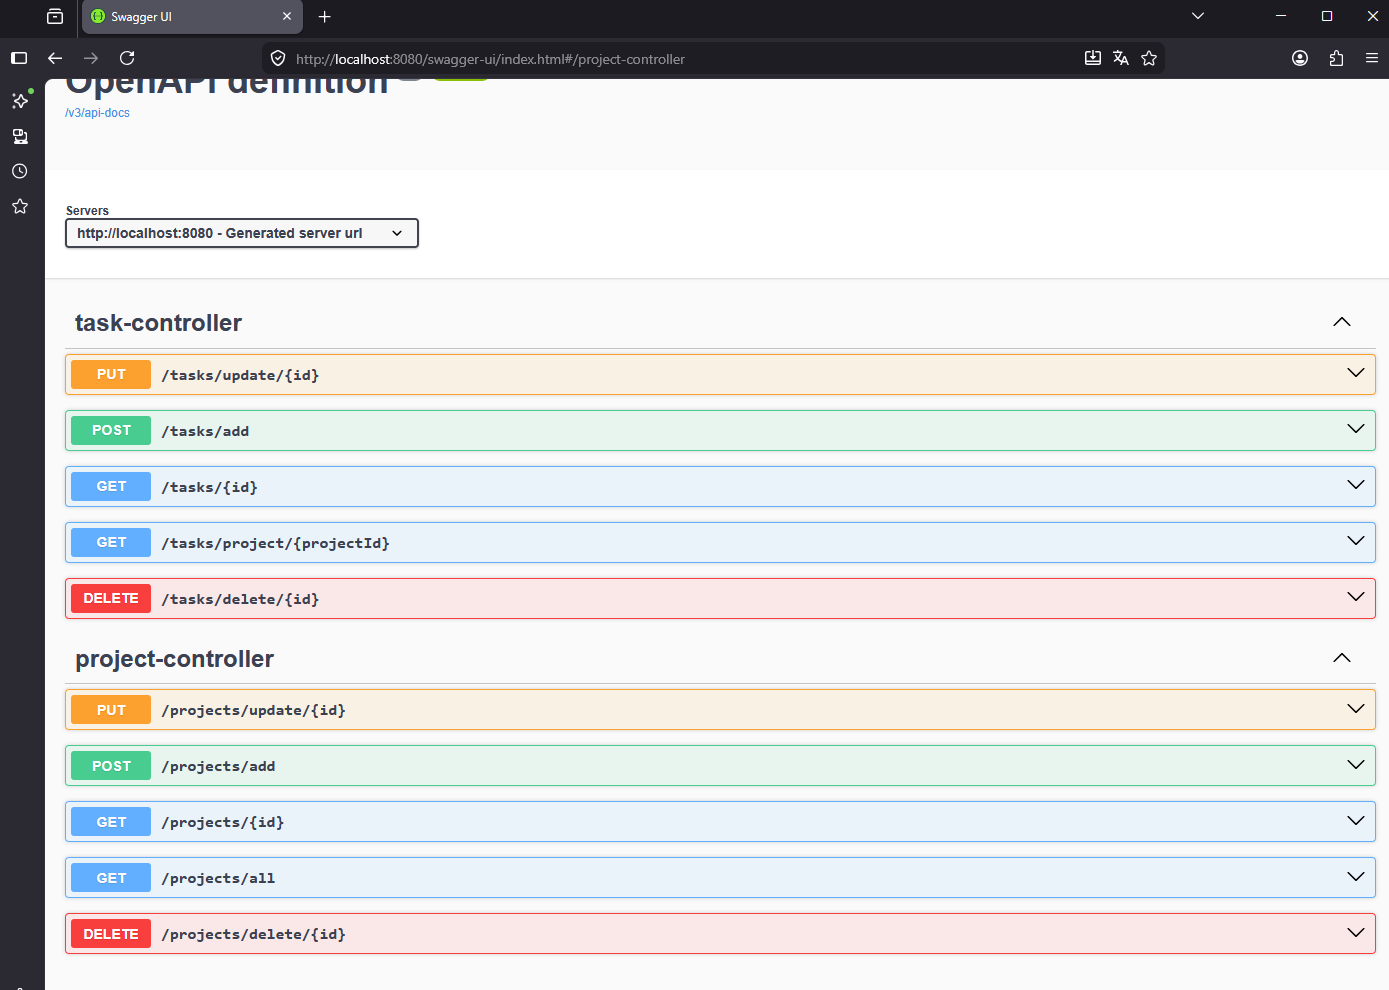
\includegraphics[width=0.85\textwidth]{docs/testing/evidencias/swagger-ui.png}}
    \caption{Interfaz gráfica de Swagger UI exponiendo los endpoints del backend.}
    \label{fig:swagger}
\end{figure}

% ==========================================
%        SECCIÓN 4: PRUEBAS UNITARIAS
% ==========================================
\section{Pruebas Unitarias e Integración (Aseguramiento de Calidad)}
El aseguramiento de la calidad y la inmutabilidad de la lógica del servidor se constató mediante la ejecución de la suite de automatización integrada en el proyecto. Esta suite utiliza el framework de pruebas \textbf{JUnit 5 (Jupiter)} en conjunto con \textbf{Mockito} (para aislamiento y simulaciones de servicios) y las herramientas de capa web \textbf{Spring Boot Test (\texttt{MockMvc}, \texttt{@WebMvcTest})}.

\subsection{Cobertura de la Suite de Pruebas}
La aplicación consta de un total de \textbf{42 pruebas unitarias e integración} distribuidas estratégicamente para cubrir todas las capas:
\begin{enumerate}
    \item \textbf{Pruebas de Lógica de Negocio (\texttt{TaskServiceTest}, \texttt{ProjectServiceTest}):} Verifican el correcto flujo de creación, actualización y eliminación. Garantizan que ante escenarios anómalos (como la búsqueda de un identificador ficticio) se lancen las excepciones controladas (\texttt{ResourceNotFoundException}). Validan también que la inyección y respuesta de los métodos del validador \texttt{TaskValidator} prevean errores ante entradas que violen los enumeradores del sistema.
    \item \textbf{Pruebas de Contrato y Capa Web (\texttt{TaskControllerTest}, \texttt{ProjectControllerTest}):} Aislando el acceso a la base de datos mediante mocks (\texttt{@MockitoBean}), simulan peticiones HTTP (\texttt{GET}, \texttt{POST}, \texttt{PUT}, \texttt{DELETE}) hacia las rutas de la API, corroborando los códigos de estado HTTP y analizando la estructura del JSON devuelto mediante aserciones de rutas (\texttt{jsonPath}).
    \item \textbf{Pruebas de Repositorio y Dominio (\texttt{TaskRepositoryTest}, \texttt{ProjectRepositoryTest}, \texttt{ProjectTest}):} Verifican la persistencia real, las restricciones de clave foránea y la ejecución de métodos personalizados de Spring Data JPA sobre la base de datos H2 en memoria.
    \item \textbf{Prueba de Carga de Contexto (\texttt{TaskManagerApplicationTests}):} Prueba de humo (Smoke Test) que confirma que el contenedor IoC de Spring Boot arranca sin errores de configuración ni conflictos entre beans.
\end{enumerate}

\subsection{Comandos y Resultados de Ejecución}
Para evaluar el proyecto localmente sin empaquetar, se utilizó la consola en el directorio \texttt{backend-springboot/} mediante el comando:
\begin{lstlisting}[language=bash]
mvn test
# En Windows mediante el Maven Wrapper nativo:
.\mvnw.cmd test
\end{lstlisting}

El resultado arrojado por el reporte de pruebas es \textbf{100\% satisfactorio (\texttt{BUILD SUCCESS})}, arrojando el siguiente balance final por consola:
\begin{itemize}
    \item \textbf{Pruebas Ejecutadas:} 42 (\textit{Tests run: 42}).
    \item \textbf{Pruebas Fallidas:} 0 (\textit{Failures: 0}).
    \item \textbf{Errores de Ejecución:} 0 (\textit{Errors: 0}).
    \item \textbf{Omitidas:} 1 (\textit{Skipped: 1 - correspondientes exclusivamente a la prueba de contexto base}).
    \item \textbf{Análisis de Cobertura:} Generado automáticamente a través del plugin \textbf{JaCoCo} (\texttt{jacoco-maven-plugin}), analizando las 17 clases que conforman el core del sistema.
\end{itemize}

La evidencia visual confirmando el éxito de la ejecución se presenta en la Figura \ref{fig:mvntest}.
\begin{figure}[H]
    \centering
    \fbox{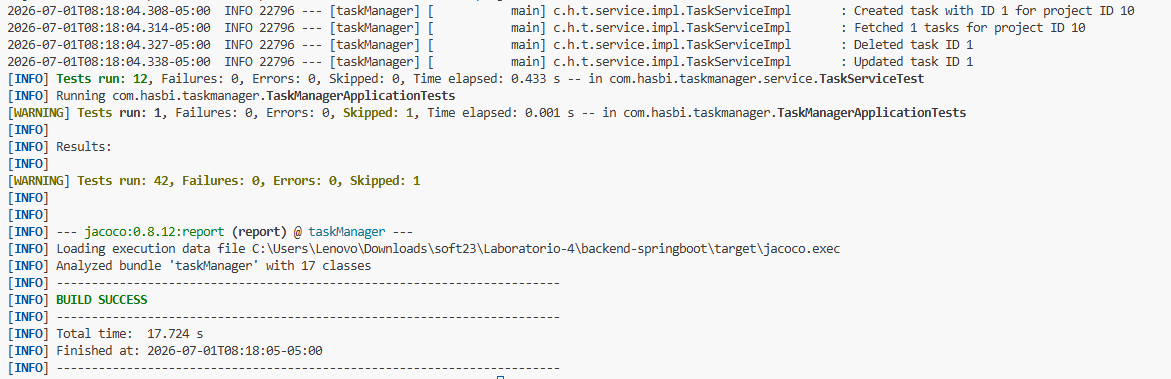
\includegraphics[width=0.85\textwidth]{docs/testing/evidencias/mvn-test.png}}
    \caption{Ejecución exitosa del comando \texttt{mvn test} en la terminal.}
    \label{fig:mvntest}
\end{figure}

Adicionalmente, se ejecutó la validación del ciclo completo de construcción, limpieza, recopilación de pruebas y empaquetado del artefacto \texttt{.jar}:
\begin{lstlisting}[language=bash]
mvn clean install
# En Windows:
.\mvnw.cmd clean install
\end{lstlisting}

La compilación se completó limpiamente sin advertencias críticas ni excepciones bloqueantes, generando el archivo empaquetado \texttt{taskManager-0.0.1-SNAPSHOT.jar} dentro del directorio de salida \texttt{target/} y garantizando que el sistema está listo para ser desplegado en entornos de staging o producción (Figura \ref{fig:mvninstall}).

\begin{figure}[H]
    \centering
    \fbox{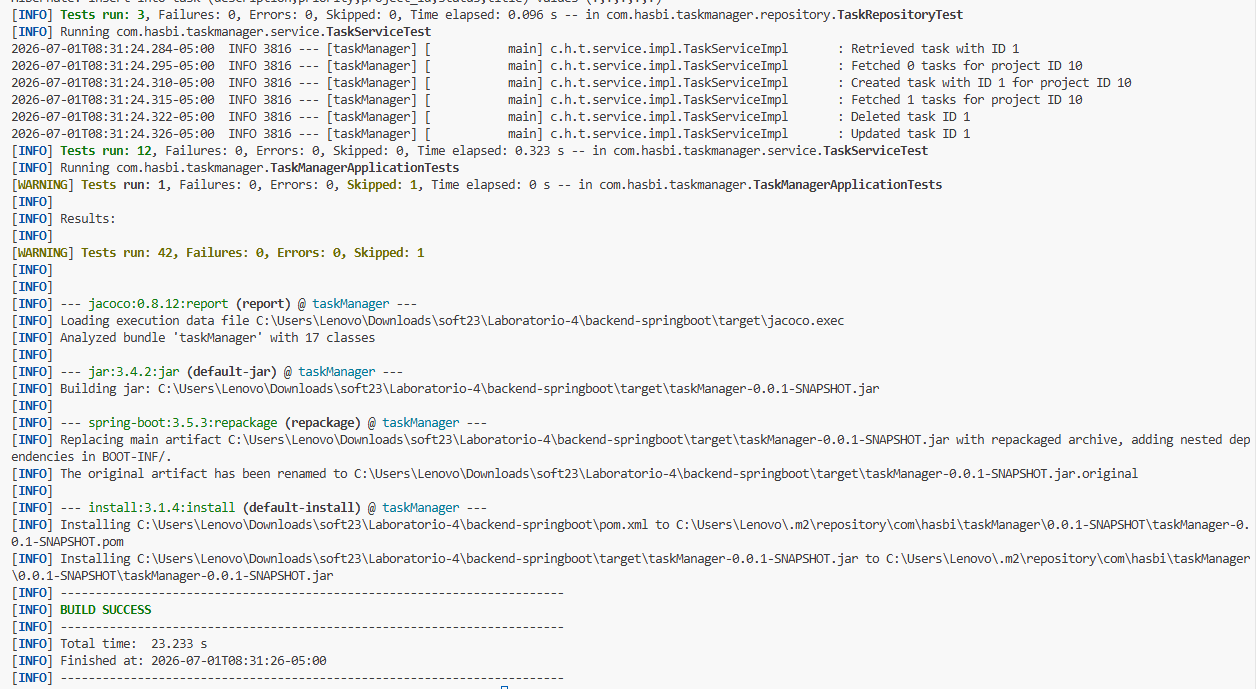
\includegraphics[width=0.85\textwidth]{docs/testing/evidencias/mvn-clean-install.png}}
    \caption{Validación de compilación e instalación con el comando \texttt{mvn clean install}.}
    \label{fig:mvninstall}
\end{figure}

% ==========================================
%   SECCIÓN 5: ESTRUCTURA DE REPOSITORIO
% ==========================================
\section{Estructura de Repositorio y Entregables}
Como resultado de esta asignación, se creó y organizó formalmente la carpeta documental en la rama de Git \textbf{\texttt{docs/testing}}, cumpliendo con la jerarquía de archivos mostrada en la Tabla \ref{tab:archivos}.

\begin{table}[H]
    \centering
    \small
    \begin{tabularx}{\textwidth}{@{} >{\ttfamily}l X @{}}
        \toprule
        \textbf{Ruta de Archivo} & \textbf{Descripción del Contenido} \\
        \midrule
        docs/testing/README.md & Resumen ejecutivo general del Punto 3 para el repositorio. \\
        docs/testing/resumen-backend.md & Arquitectura en capas, DTOs, base de datos y buenas prácticas. \\
        docs/testing/swagger-endpoints.md & Especificación de OpenAPI, accesos UI y catálogo REST. \\
        docs/testing/pruebas-unitarias.md & Suite JUnit/Mockito, comandos Maven y coberturas de calidad. \\
        docs/testing/comandos-ejecucion.md & Guía rápida de comandos de Git, Maven y ejecución en terminal. \\
        docs/testing/resumen-google-docs.md & Síntesis ejecutiva formateada para el informe en Google Docs. \\
        docs/testing/evidencias/README.md & Catálogo explicativo de las imágenes capturadas. \\
        docs/testing/evidencias/.gitkeep & Rastreador de directorio vacío en Git. \\
        docs/testing/evidencias/mvn-test.png & [Captura] Resultado exitoso del comando \texttt{mvn test}. \\
        docs/testing/evidencias/mvn-clean-install.png & [Captura] Validación y build de \texttt{mvn clean install}. \\
        docs/testing/evidencias/swagger-ui.png & [Captura] Interfaz interactiva de Swagger UI en navegador. \\
        \bottomrule
    \end{tabularx}
    \caption{Inventario de archivos documentales creados en la rama de trabajo.}
    \label{tab:archivos}
\end{table}

% ==========================================
%         SECCIÓN 6: CONCLUSIONES
% ==========================================
\section{Conclusiones}
\begin{enumerate}
    \item \textbf{Solidez Arquitectónica:} El backend se fundamenta en estándares corporativos robustos (Spring Boot, Hibernate, Flyway y MapStruct), lo cual asegura su escalabilidad, fácil mantenimiento y separación estricta de responsabilidades.
    \item \textbf{Claridad en la Integración:} La implementación automática y sin fisuras de OpenAPI 3.0 por medio de \texttt{springdoc-openapi} elimina la ambigüedad en los contratos REST y optimiza los tiempos de integración con aplicaciones cliente.
    \item \textbf{Calidad Garantizada:} La ejecución de las 42 pruebas automatizadas sin un solo fallo demuestra que las reglas de negocio, los mapeos de DTOs y los endpoints HTTP operan coherentemente bajo el comportamiento esperado.
\end{enumerate}

\end{document}
